\documentclass[./thesis.tex]{subfiles}

\begin{document}

In this chapter, we discuss the efficiency of the implementation. The system
we chose for these numerical experiments is a cyanine dye, \\
\begin{center}
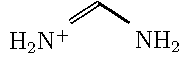
\includegraphics[]{figures/perf/Cyanine} \\
\end{center}
%[(NH$_2$)(CH)(NH$_2$)]$^+$
in its ground state and in its first excited state.
The geometry is the equilibrium geometry of the ground state, optimized at the
PBE0/cc-pVQZ level. The ground state is a closed shell, well described by a
single reference, and the excited state is singly excited and requires two
determinants in the reference ($1/\sqrt{2} (a\bar{b} + b\bar{a})$).  The
calculations were performed in the aug-cc-pVDZ basis set with state-averaged
natural orbitals obtained from an initial CIPSI calculation.
The $1s$ orbitals of the carbon and the nitrogen atoms were frozen, so
the FCI space which is explored is a CAS(18,111). The reference excitation
energy, obtained at the CC3/ANO-L-VQZP level is 7.18~eV.\cite{Send_2011}
The measurements were made on the Olympe supercomputer (CALMIP). Each node is 
a dual-socket Intel(R) Xeon(R) Gold 6140 CPU @ 2.30GHz with 192GiB of RAM, and
contains 36 physical CPU cores.

\begin{figure}[hbt]
	\begin{center}
		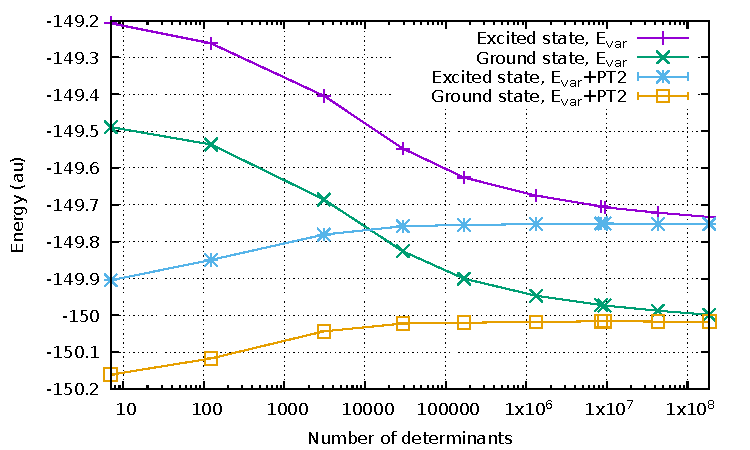
\includegraphics[width=0.8\columnwidth]{figures/perf/cn3_energy}
		\caption{Convergence of the energy of the ground and excited states with respect to the number of determinants in the variational space.}
		\label{fig:energy_pt2}
	\end{center}
\end{figure}

\begin{table}[hbt]
\caption{Energies and second-order perturbative corrections for increasingly large wave functions. $\Delta$ is the energy difference
between the ground state and the excited state.}
\label{tab:energy_pt2}
\begin{center}
\begin{tabular}{rllrr}
\hline
\tabc{$\Ndet$} & \tabc{Ground state} & \tabc{Excited state} & \tabc{$\Delta E$ (eV)} \\
\hline
\multicolumn{4}{c}{$\Evar$}  \\
$          7$ & $-149.489~186$ & $-149.207~354$ & $7.67$  \\
$        123$ & $-149.536~265$ & $-149.261~860$ & $7.47$  \\
$      3~083$ & $-149.685~606$ & $-149.404~450$ & $7.65$  \\
$     29~409$ & $-149.826~151$ & $-149.547~275$ & $7.59$  \\
$    168~595$ & $-149.900~352$ & $-149.626~058$ & $7.46$  \\
$  1~322~537$ & $-149.946~655$ & $-149.675~032$ & $7.39$  \\
$  8~495~334$ & $-149.972~032$ & $-149.704~145$ & $7.29$  \\
$  9~356~952$ & $-149.973~375$ & $-149.706~822$ & $7.25$  \\
$ 42~779~636$ & $-149.987~370$ & $-149.721~470$ & $7.24$  \\
$186~978~487$ & $            $ & $            $ & $7.22$  \\
\hline

\multicolumn{4}{c}{$\Evar + \EPT$}  \\
$          7$ & $-150.161~107  $ & $-149.904~883  $ & $6.97$ \\
$        123$ & $-150.116~958  $ & $-149.849~465  $ & $7.28$ \\
$      3~083$ & $-150.043~5(2) $ & $-149.780~8(2) $ & $7.15$ \\
$     29~409$ & $-150.022~2(2) $ & $-149.758~3(2) $ & $7.18$ \\
$    168~595$ & $-150.019~9(1) $ & $-149.754~5(1) $ & $7.22$ \\
$  1~322~537$ & $-150.017~89(7)$ & $-149.752~55(7)$ & $7.22$ \\
$  8~495~334$ & $-150.015~97(4)$ & $-149.750~87(5)$ & $7.21$ \\
$  9~356~952$ & $-150.015~95(4)$ & $-149.750~68(4)$ & $7.22$ \\
$ 42~959~496$ & $-150.016~75(2)$ & $-149.751~88(2)$ & $7.21$ \\
\hline
\end{tabular}
\end{center}
\end{table}

In figure~\ref{fig:energy_pt2}, we plot the convergence of the energies of
the ground and excited states as a function of the number of
determinants, with and without the second order perturbative contribution.
From these data, one can see that although $\EPT$ is still large ($\sim 0.04$~au)
the excitation energies both at the variational level and with the perturbative
correction converge to a value of $7.21$~eV compatible with the reference
energy obtained in a larger basis set.



\clearpage

\section{Davidson diagonalization}

\begin{table}[hbt]
\caption{Wall-clock time (in seconds) to run one Davidson's iteration in parallel with increasingly large wave functions.}
\label{tab:time_davidson_ndet}
\begin{center}
\begin{tabular}{rr}
\hline
\tabc{$\Ndet$} & \tabc{seconds} \\
\hline
$    29~409$ &       $0.91$ \\
$   168~595$ &       $7.15$ \\
$ 1~322~537$ &      $59.32$ \\
$ 8~495~334$ &     $802.02$ \\
$ 9~356~952$ &     $955.58$ \\
$42~959~496$ &  $12~361.68$ \\
\hline
\end{tabular}
\end{center}
\end{table}

\begin{table}[hbt]
\caption{Wall-clock time (in seconds) to run one Davidson's iteration in parallel on two different wave functions 
with an increasing number of 36-core compute nodes.}
\label{tab:time_davidson}
\begin{center}
\begin{tabular}{rrr}
\hline
\tabc{Nodes} & \tabc{9~356~952 determinants} & \tabc{42~959~496 determinants} \\
\hline
$ 1$ &$955.58$ &$12~361.68$\\
$ 5$ &$215.02$ &$ 2~580.71$\\
$10$ &$121.28$ &$ 1~363.25$\\
$20$ &$ 75.59$ &$   746.36$\\
$30$ &$ 61.42$ &$   542.92$\\
$40$ &$ 51.97$ &$   442.12$\\
$50$ &$ 48.66$ &$   381.92$\\
\hline
\end{tabular}
\end{center}
\end{table}

\begin{figure}[h]
    \begin{center}
      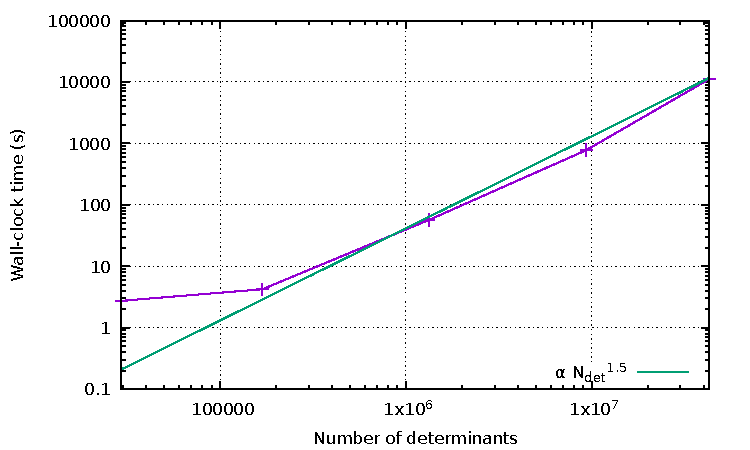
\includegraphics[width=0.8\columnwidth]{figures/perf/scaling_davidson_ndet}
      \caption{Wall-clock time of one Davidson iteration as a function of the number of
determinants in the wave function.}
      \label{fig:speedup_davidson_ndet}
    \end{center}
\end{figure}

\begin{figure}[h]
    \begin{center}
      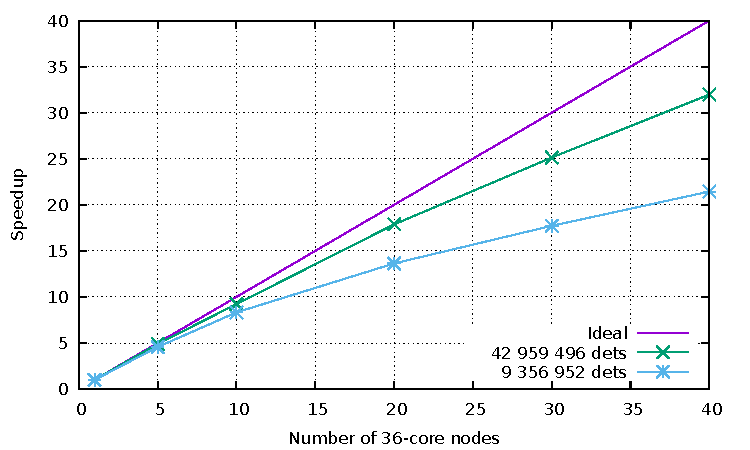
\includegraphics[width=0.8\columnwidth]{figures/perf/scaling_davidson}
      \caption{Speedup of one Davidson iteration as a function of the number of
36-core compute nodes.}
      \label{fig:speedup_davidson}
    \end{center}
\end{figure}

We took a wave function with 42~959~496 determinants, and measured the wall-clock time required to
perform one iteration of the Davidson diagonalization, with an increasing number of compute nodes.
The timings are reported in table~\ref{tab:time_davidson} and the parallel speedup curve is represented in figure~\ref{fig:speedup_davidson}.


\clearpage

\section{Selection}

\begin{table}[hbt]
\caption{Single-node (36-core) CIPSI selection for increasingly large wave functions. Time is given in seconds.}
\label{tab:time_selection}
\begin{center}
\begin{tabular}{rr}
\hline
\tabc{$\Ndet$} & \tabc{seconds} \\
\hline
$      123$ & $     0.18$ \\
$    3~083$ & $     6.23$ \\
$    7~036$ & $    16.32$ \\
$   17~174$ & $    40.46$ \\
$   40~692$ & $   102.76$ \\
$   98~186$ & $   253.56$ \\
$  240~422$ & $   654.87$ \\
$  639~269$ & $ 1~802.61$ \\
$1~928~131$ & $ 5~258.16$ \\
\hline
\end{tabular}
\end{center}
\end{table}

\begin{table}[hbt]
\caption{Time (in seconds) to run parallel CIPSI selections on the
9~356~952-determinant wave function with an increasing number of 36-core
compute nodes.}
\label{tab:selection_parallel}
\begin{center}
\begin{tabular}{rr}
\hline
\tabc{Nodes} & \tabc{seconds}  \\
\hline
$ 1$ & $14~945.80$ \\
$ 5$ & $ 3~419.55$ \\
$10$ & $ 1~655.23$ \\
$20$ & $   943.97$ \\
$30$ & $   748.88$ \\
$40$ & $   666.26$ \\
$50$ & $   748.99$ \\
\hline
\end{tabular}
\end{center}
\end{table}

\begin{figure}[hbt]
    \begin{center}
      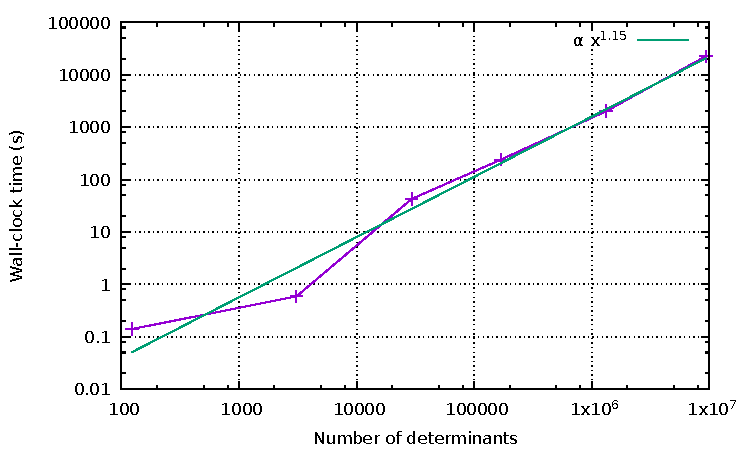
\includegraphics[width=0.8\columnwidth]{figures/perf/scaling_sel_det}
      \caption{Wall-clock time of the selection as a function of the number of
determinants in the wave function.}
      \label{fig:scaling_sel_ndet}
    \end{center}
\end{figure}

\begin{figure}[h]
    \begin{center}
      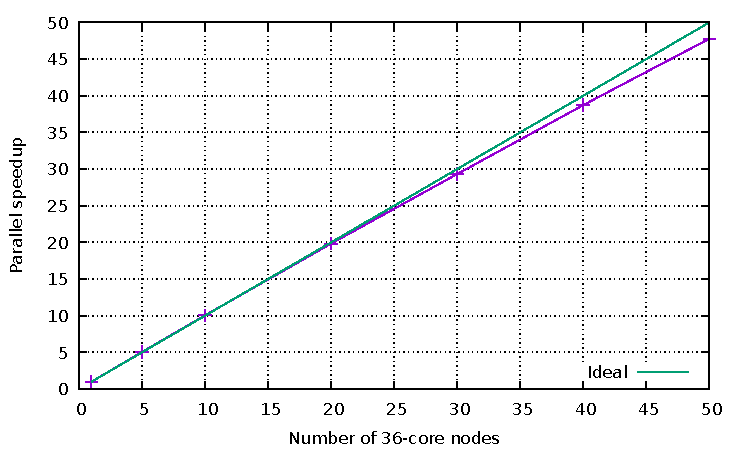
\includegraphics[width=0.8\columnwidth]{figures/perf/scaling_sel_node}
      \caption{Parallel speedup of the CIPSI selection. The reference is a single 36-core node.}
      \label{fig:speedup_sel_node}
    \end{center}
\end{figure}

We have measured the time necessary to realize a selection step, with an
increasing number of determinants in the variational space.
Figure~\ref{fig:scaling_sel_node} shows a linear scaling with the number of
determinants. The parallel speedup was also measured with up to 50 nodes, but
the maximum speedup value is $\sim 20$ with 40 nodes. This is explained by
the overall low computational cost of the algorithm (a small wall-clock time), 
and communications scaling as $\order{\Ndet}$, as the computation.




\clearpage

\section{PT2 calculations}

The stopping criterion of the calculation of the PT2 contribution was a
relative statistical error below 1/1000-th.
The fraction of the full deterministic calculation required to reach this criterion
is typically around $5\%$.

\begin{figure}[hbt]
	\begin{center}
		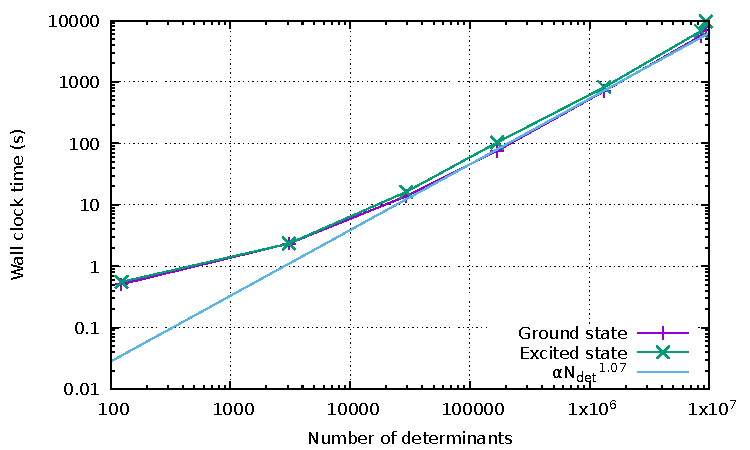
\includegraphics[width=0.8\columnwidth]{figures/perf/scaling_pt2_det}
		\caption{Wall clock time required to compute $\EPT$ for the ground and the excited states, as a function of the number of determinants in the wave function.}
		\label{fig:scaling_det_pt2}
	\end{center}
\end{figure}

\begin{table}[hbt]
\caption{Single-node (36-core) $\EPT$ calculations for increasingly large wave functions. Time is given in seconds.}
\label{tab:time_pt2}
\begin{center}
\begin{tabular}{rrr}
\hline
\tabc{$\Ndet$} & \tabc{Ground state} & \tabc{Excited state} \\
\hline
$      123$ &  $     0.48$ & $     0.53$ \\
$    3~083$ &  $     1.53$ & $     2.05$ \\
$   29~409$ &  $    13.71$ & $    23.75$ \\
$  168~595$ &  $   138.17$ & $   155.36$ \\
$1~322~537$ &  $ 2~456.66$ & $ 2~640.67$ \\
$8~495~334$ &  $38~350.47$ & $42~796.15$ \\
$9~356~952$ &  $44~873.53$ & $50~361.70$ \\
\hline
\end{tabular}
\end{center}
\end{table}

Table~\ref{tab:time_pt2} reports the wall-clock time required to compute $\EPT$
on a single node.
From these data, one can evaluate the scaling of the cost of $\EPT$ 
with the number of determinants, as plotted in figure~\ref{fig:scaling_det_pt2}.

The number of $\ket{\alpha}$ determinants is proportional to the
number of determinants in the variational wave function, and each
$\ket{\alpha}$ needs to be compared to all the determinants 
in the computation of $\mel{\alpha}{H}{\Psi}$.
But when the wave function becomes large enough, the second point is not true any more because only a limited number of determinants $\ket{I}$ of $\Psi$ have a non-zero
value $\mel{\alpha}{H}{I}$, and this number is bounded by the number of single and double excitations, characteristic of the basis set.
Fitting the last points with a log-log plot shows an asymptotic scaling as
$\order{\Ndet^{1.45}}$, which is consistent with the fact that the scaling is
expected to be going from $\order{\Ndet^2}$ for small sizes to $\order{\Ndet}$.


\begin{table}
\caption{Time (in seconds) to run parallel $\EPT$ calculations on the largest wave function with an
increasing number of 36-core compute nodes.}
\label{tab:pt2_parallel}
\begin{center}
\begin{tabular}{rrr}
\hline
\tabc{Nodes} & \tabc{Ground state} & \tabc{Excited state} \\
\hline
$ 1$ & $44~873.53$ & $50~361.70$ \\
$ 5$ & $10~552.02$ & $11~260.12$ \\
$10$ & $ 5~381.51$ & $ 5~918.34$ \\
$20$ & $ 2~782.87$ & $ 3~043.94$ \\
$30$ & $ 1~884.67$ & $ 2~069.17$ \\
$40$ & $ 1~440.96$ & $ 1~568.30$ \\
$50$ & $ 1~154.97$ & $ 1~273.66$ \\
\hline
\end{tabular}
\end{center}
\end{table}
\begin{figure}[hbt]
	\begin{center}
		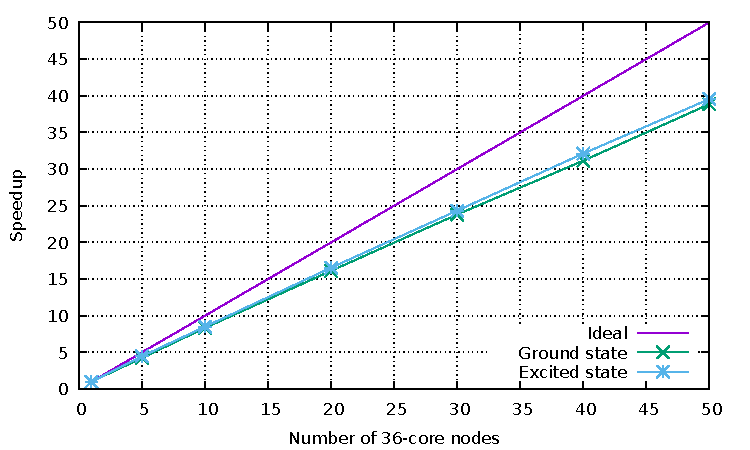
\includegraphics[width=0.8\columnwidth]{figures/perf/scaling_pt2_node}
		\caption{Parallel speedup for the calculation of the $\EPT$ contribution of the ground state using the largest wave function. Each node contains 36 physical CPU cores.}
		\label{fig:scaling_node_pt2}
	\end{center}
\end{figure}

To analyze the parallel efficiency of the $\EPT$ calculation, we have made the parallel speedup curve using up to 50 nodes (1800 CPU cores), plotted in figure~\ref{fig:scaling_node_pt2}. With 50 nodes, one obtains a speedup with respect to the single-node reference of $38.8\times$ for the ground state and $39.5\times$ for the excited state. This corresponds to a parallel efficiency of 77.7\% and 79.1\%.

\clearpage

\section{Shifted-Bk}

\begin{table}[hbt]
\caption{Single-node (36-core) Shifted-$B_k$ iteration for increasingly large wave functions.
Time is given in seconds.}
\label{tab:time_selection}
\begin{center}
\begin{tabular}{rr}
\hline
\tabc{$\Ndet$} & \tabc{Ground state} & \tabc{Excited state} \\
\hline
$      123$ & $     0.24$  & $     0.81$ \\
$    3~083$ & $     3.79$  & $     4.75$ \\
$   29~409$ & $    23.12$  & $    28.72$ \\
$  168~595$ & $   200.06$  & $   219.91$ \\
$1~322~537$ & $  2784.19$  & $  3023.61$ \\
$9~356~952$ & $ 27476.91$  & $ 28253.20$ \\
\hline
\end{tabular}
\end{center}
\end{table}
\begin{figure}[hbt]
	\begin{center}
		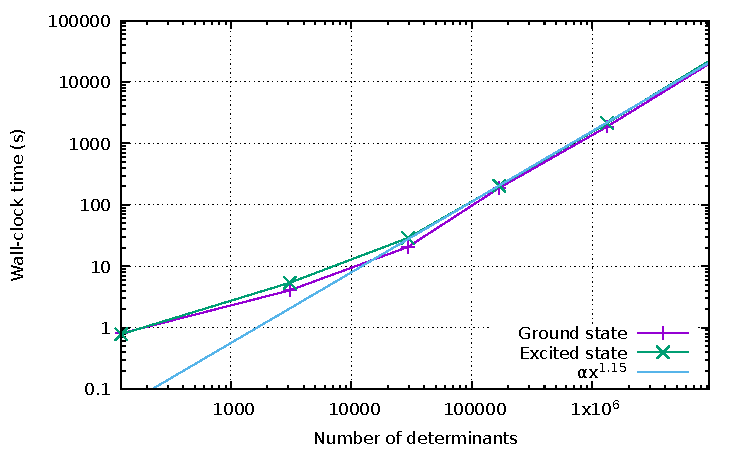
\includegraphics[width=0.8\columnwidth]{figures/perf/scaling_sbk_det}
		\caption{Wall clock time required to compute the Shifted-$B_k$ dressing for the ground and the excited states, as a function of the number of determinants in the wave function.}
		\label{fig:scaling_det_sbk}
	\end{center}
\end{figure}

The time necessary to build the dressing matrix in the Shifted-$B_k$ method was measured on a single
36-core node with an increasing number of determinants (figure~\ref{fig:scaling_det_sbk}).
The stopping criterion was an estimated relative error on 
$\mel{\Psi}{\hat \Delta}{\Psi}$, the dressed energy, equal to $0.01$.

Using the log-log plot, the scaling with the number of determinants was found to be
$\order{\Ndet^{1.25}}$. In the previous section, we have seen that the scaling for $\EPT$ was
$\order{\Ndet^{1.5}}$. We can explain this difference by the fact that in the 
calculation of $\EPT$, the communication was negligible. In the computation of the
matrix dressing, the result of each task scales as $\order{\Ndet}$. To palliate this 
bottleneck, the results of multiple tasks are aggregated together and one large message is
sent at every checkpoint. The computational overhead for this reduction of the communication
scales as $\order{\Ndet}$, and this explains why the scaling with the number of determinants is
closer to linear than for $\EPT$.

\begin{figure}[hbt]
	\begin{center}
		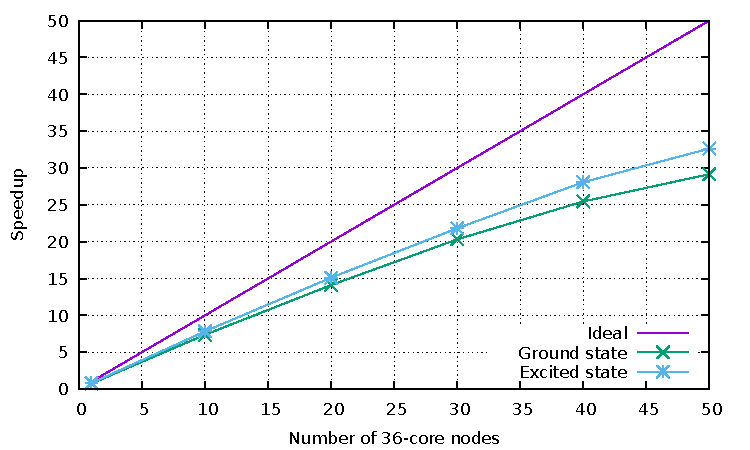
\includegraphics[width=0.8\columnwidth]{figures/perf/scaling_sbk_node}
		\caption{Parallel speedup for the calculation of the matrix dressing of the ground state using the largest wave function. Each node contains 36 physical CPU cores.}
		\label{fig:scaling_node_sbk}
	\end{center}
\end{figure}

Then, the parallel speedup was measured using the wavefunction with 9~356~952 determinants. The results
are plotted in figure~\ref{fig:scaling_node_sbk}.

\clearpage

\section{Multi-reference Coupled-Cluster}

\end{document}
